\title{Esercitazione 2 26/03/2020}\newline
\textbf{link} \href{https://web.microsoftstream.com/video/c4d111d7-4825-4513-afe0-f0fd323398dd}{Clicca qui}
\section{Esercitazione II}
\url{../esercitazione2/pdf/02-Cinematica cr disco - moti relativi gru.pdf}\newline
\url{../esercitazione2/pdf/ese_2_notes.pdf}\newline
\subsection{Ripasso sulla cinematica del corpo rigido}
Definito un corpo rigido e due sue punti interni $A$ e $B$, allora il \textbf{teroema di Rivals della velocità} dice che:
\[
    \vec{v}_B = \vec{v}_A + \vec{v}_{BA} = \vec{v}_A + \vec{\omega} \land (B-A)
\]
con $\vec{v}_{BA}$ velocità di $B$ in moto circolare visto da un osservatore traslante in $A$.\newline
\newline
Il \textbf{centro di istantanea rotazione} (CIR) è un punto che nell'istante in cui viene osservato ha velocità nulla. Mentre un \textbf{centro di rotazione} ha velocità nulla in ogni istante e quindi anche accellerazione nulla.\newline
\newline
Il \textbf{teorema di Rivals dell'accellerazione} dice che:
\[
    \vec{a}_B = \vec{a}_A + \dot{\vec{\omega}} \land (B-A) + \vec{\omega} \land [\vec{\omega} \land (B-A)] = \vec{a}_A + \dot{\vec{\omega}} \land (B-A) - \omega^2 (B-A)
\]
dove $\vec{a}_{BA} = \dot{\vec{\omega}} \land (B-A) - \omega^2 (B-a)$ è l'accellerazione di $B$ vista da un osservatore traslante in $A$.
\subsection{Ripasso sui moti relativi}
Definita una terna fissa $X_0 O_0 Y_0$ e una terna rototraslante $X_1O_1Y_1$ per descrivere il moto di un punto $P$ nello spazio.\newline
[immagine dagli appunti del prof]
\begin{center}
    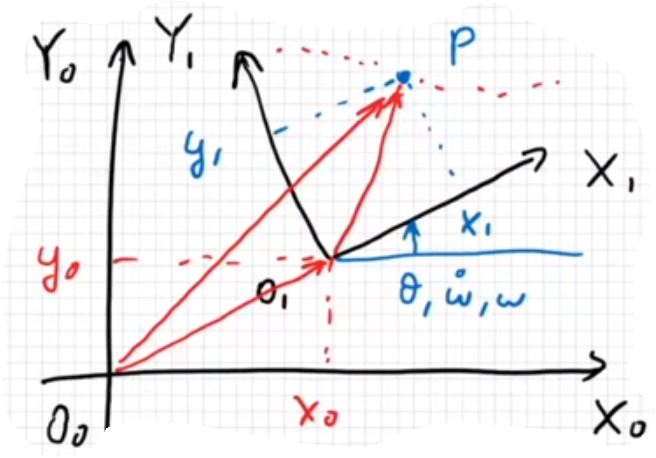
\includegraphics[height=3cm]{../esercitazione2/img1.JPG}
\end{center}
\textbf{Velocità}:
\[
    \vec{v}_P^{(0)} = \vec{v}_{O_1} + \vec{\omega} \land (P-O_1) + v_{rel,P}^{(1)}
\]
dove $\vec{v}_P^{(0)}$ è la \textbf{velocità assoluta}, $\vec{v}_{O_1} + \vec{\omega} \land (P-O_1)$ è la \textbf{velocità di trascinamento (traslatoria-rotatoria)}, e $v_{rel,P}^{(1)}$ è la \textbf{velocità relativa}.\newline
\newline
\textbf{Accellerazione}:
\[
    \vec{a}_P^{(0)} = \vec{a}_{O_1} + \dot{\vec{\omega}} \land (P-O_1) + \vec{\omega} \land [\vec{\omega} \land (P-O_1)] + \vec{a}_{rel,P} + 2 \vec{\omega} \land \vec{v}_{rel,P}
\]
dove $\vec{a}_P^{(0)}$ è l'\textbf{accellerazione assoluta}, $\vec{a}_{O_1} + \dot{\vec{\omega}} \land (P-O_1) + \vec{\omega} \land [\vec{\omega} \land (P-O_1)]$ è l'\textbf{accellerazione di trascinamento}, $\vec{a}_{rel,P}$ è l'\textbf{accellerazione relativa}, e $2 \vec{\omega} \land \vec{v}_{rel,P}$ è l'\textbf{accellerazione di Coriolis}.